 %\pdfoutput=1
\documentclass[%
 reprint,
%superscriptaddress,
%groupedaddress,
%unsortedaddress,
%runinaddress,
%frontmatterverbose, 
%preprint,
%preprintnumbers,
%nofootinbib,
%nobibnotes,
%bibnotes,
 amsmath,amssymb,
 aps,
prd,
%prb,
%rmp,
%prstab,
%prstper,
%floatfix,
]{revtex4-2}
%\usepackage{jheppub}
%\usepackage{ctex}

\usepackage{fix-cm}
\usepackage{amsfonts}
\usepackage{mathrsfs}
\usepackage{amsmath}
\usepackage{amssymb}
\usepackage{framed}

%\usepackage[medium]{titlesec}
\usepackage{bm}

\usepackage[normalem]{ulem}
\usepackage{extarrows}
\usepackage{slashed}
\usepackage{isodateo}
\usepackage{graphicx}
\usepackage[dvipsnames]{xcolor}
%\usepackage[bookmarksnumbered=true,bookmarksopen=true]{hyperref}
%\hypersetup{colorlinks,%
%             linkcolor=NavyBlue, %
%             citecolor=PineGreen, %
%             urlcolor=PineGreen}
%\usepackage[hmargin=.7in,vmargin=1.1in]{geometry}
\usepackage{indentfirst,comment}
\usepackage{booktabs}

\usepackage{bbm}
\usepackage{tikz-cd}
\usetikzlibrary{patterns}
\usepackage{tikz}
\usetikzlibrary{arrows,shapes}
\usetikzlibrary{trees}
\usetikzlibrary{matrix,arrows} 				% For commutative diagram
% http://www.felixl.de/commu.pdf
\usetikzlibrary{positioning}				% For "above of=" commands
\usetikzlibrary{calc,through}				% For coordinates
\usetikzlibrary{decorations.pathreplacing}  % For curly braces
% http://www.math.ucla.edu/~getreuer/tikz.html
\usepackage{pgffor}							% For repeating patterns

\usetikzlibrary{decorations.pathmorphing}	% For Feynman Diagrams
\usetikzlibrary{decorations.markings}
\tikzset{
	% >=stealth', %%  Uncomment for more conventional arrows
	photon/.style={decorate, decoration={snake}, draw=red},
	electron/.style={draw=blue, postaction={decorate},
		decoration={markings,mark=at position .55 with {\arrow[draw=blue]{>}}}},
	gluon/.style={decorate, draw=blue,
		decoration={coil,amplitude=4pt, segment length=4pt}} ,
	vector/.style={decorate, decoration={snake}, draw},
	provector/.style={decorate, decoration={snake,amplitude=2.5pt}, draw},
	antivector/.style={decorate, decoration={snake,amplitude=-2.5pt}, draw},
	fermion/.style={draw=black, postaction={decorate},
		decoration={markings,mark=at position .55 with {\arrow[draw=black]{>}}}},
	fermionbar/.style={draw=black, postaction={decorate},
		decoration={markings,mark=at position .55 with {\arrow[draw=black]{<}}}},
	fermionnoarrow/.style={draw=black},
	%    gluon/.style={decorate, draw=black,
	%        decoration={coil,amplitude=3pt, segment length=5pt}},
	%gluon/.style={decorate, draw=magenta,
	%	decoration={coil,amplitude=4pt, segment length=5pt}},
	scalar/.style={draw=black, postaction={decorate},
		decoration={markings,mark=at position .55 with {\arrow[draw=black]{>}}}},
	scalarbar/.style={dashed,draw=black, postaction={decorate},
		decoration={markings,mark=at position .55 with {\arrow[draw=black]{<}}}},
	scalarnoarrow/.style={dashed,draw=black},
	electron/.style={draw=black, postaction={decorate},
		decoration={markings,mark=at position .55 with {\arrow[draw=black]{>}}}},
	bigvector/.style={decorate, decoration={snake,amplitude=4pt}, draw},
	background/.style={dashed,draw=black, postaction={decorate},
		decoration={markings,mark=at position 1 with {\arrow[draw=black]{<>}}}},
	%	line/.style={markings,draw=black},
	%	green/.style={draw=black, postaction={decorate}},
}

% TIKZ - for block diagrams, 
% from http://www.texample.net/tikz/examples/control-system-principles/
% \usetikzlibrary{shapes,arrows}
\tikzstyle{block} = [draw, rectangle, 
minimum height=3em, minimum width=6em]
%\linespread{1.1}

\definecolor{lightgreen}{cmyk}{0.2, 0, 0.2, 0.2}
\definecolor{lightgray}{cmyk}{0.1,0.2,0,0.1}
\definecolor{lightgray2}{cmyk}{0.1,0.1,0,0.1}
\definecolor{greyish2}{rgb}{.96,.96,.96}
\definecolor{bluecyan}{RGB}{0, 100, 200}
\definecolor{blue3}{RGB}{31,119,180}
\definecolor{red3}{RGB}{214,39,40}
\definecolor{orange3}{RGB}{255,127,14}
\definecolor{green3}{RGB}{44,160,44}
\definecolor{red2}{RGB}{255,0,0}
\definecolor{green2}{RGB}{0,170,0}
\definecolor{blue2}{RGB}{0,128,255}
\definecolor{magenta2}{RGB}{191,64,191}
\definecolor{purple2}{RGB}{112,48,160}
\definecolor{orange2}{RGB}{255,192,0}
\definecolor{blue2}{RGB}{117,223,230}
\definecolor{red4}{RGB}{186,60,71}


\newcommand{\fr}[2]{\mbox{$\frac{\,{#1}\,}{#2}$}}
\newcommand{\n}{\nonumber}
\renewcommand{\rm}{\mathrm}
\renewcommand{\thefootnote}{\arabic{footnote}}

\graphicspath{{fig/}}


\newcommand{\red}{\color{red}}
\newcommand{\blue}{\color{blue}}
\newcommand{\gray}{\color{gray}}

\def\bge{\begin{equation}}
\def\ede{\end{equation}}
\def\bga{\begin{aligned}}
\def\eda{\end{aligned}}
\def\ie{\begin{equation}\begin{aligned}}
\def\fe{\end{aligned}\end{equation}}
\def\bgb{\begin{bmatrix}}
\def\edb{\end{bmatrix}}
\def\bgp{\begin{pmatrix}}
\def\edp{\end{pmatrix}}
\def\bgm{\begin{matrix}}
\def\edm{\end{matrix}}
\def\bgs{\begin{subequations}}
\def\eds{\end{subequations}}
\def\di{{\mathrm{d}}}

\def\mb{\mathbf}
\def\pd{\partial}
\def\tr{\mathrm{\,tr\,}}
\def\Tr{\mathrm{\,Tr\,}}
\def\Det{\mathrm{\,Det\,}}


\def\To{\Rightarrow}
\def\ii{\mathrm{i}}

\def\ep{\epsilon}

\def\aa{\mathsf{a}}
\def\bb{\mathsf{b}}
\def\cc{\mathsf{c}}
\def\dd{\mathsf{d}}

\newcommand{\mN}{\mathcal{N}}
\newcommand{\mG}{\mathcal{G}}
\newcommand{\mK}{\mathcal{K}}
\def\to{\rightarrow}



\def\Re{\mathrm{Re}\,}
\def\Im{\mathrm{Im}\,}

\def\ad{\mathrm{\,ad\,}}

\def\2F1{{}_2\mathrm{F}_1}
\def\3F2{{}_3\mathrm{F}_2}

\def\nut{\wt{\nu}}
%\newcommand{\nut}{\widetilde{\nu}}


\def\tf{{\tau_0}}

\usepackage{mdframed} 
                   

\newmdenv[skipabove=0pt,%
skipbelow=5pt,%
leftmargin=0pt,%
rightmargin=0pt,%
innertopmargin=-5pt,%
innerbottommargin=7pt,%
innerleftmargin=2pt,%
innerrightmargin=2pt,%
splittopskip=0pt,%
splitbottomskip=0pt,%
linewidth=0pt,%
nobreak=true]%
{keyeqn2}                   


\newmdenv[backgroundcolor=gray!15,%
skipabove=0pt,%
skipbelow=5pt,%
leftmargin=0pt,%
rightmargin=0pt,%
innertopmargin=-5pt,%
innerbottommargin=7pt,%
innerleftmargin=2pt,%
innerrightmargin=2pt,%
splittopskip=0pt,%
splitbottomskip=0pt,%
linewidth=0pt,%
nobreak=true]%
{keyeqn}
          
%\usepackage{titlesec}          
%\titleformat{\section}
%{\normalfont\fontsize{15}{20}\bfseries}{\thesection}{1em}{}

\newcommand{\ob}[1]{\mkern 2mu \overline{\mkern -2mu #1 \mkern -2mu}\mkern 2mu}
\newcommand{\wt}[1]{\mkern 2mu \widetilde{\mkern -2mu #1 \mkern -2mu}\mkern 2mu}
\newcommand{\wh}[1]{\mkern 2mu \widehat{\mkern-2mu#1\mkern-2mu}\mkern 2mu}

\newcommand{\fnemail}[1]{\footnote{Email: \href{mailto:#1}{\nolinkurl{#1}}}}


\newcommand{\zq}[1]{{\color[rgb]{.1,.6,.3}{[{ZQ:} #1]}}}
\newcommand{\cjq}[1]{{\color[rgb]{.1,.6,.3}{[{CJQ:} #1]}}}
\newcommand{\tyx}[1]{{\color[rgb]{.1,.6,.3}{[{YT:} #1]}}}
\begin{document}

\title{dS loop integrals: The parity-split IBP system and $\di\log$-form differential equation by intersection theory}





\author{Jiaqi Chen$^{1,2}$}
\email{jiaqichen@cup.edu.cn}

\author{Bo Feng$^{3}$}
\email{fengbo@scnu.edu.cn}

\author{Zhehan Qin$^{4}$}
\email{qzh21@mails.tsinghua.edu.cn}

\author{Yi-Xiao Tao$^{5}$}
\email{taoyx21@mails.tsinghua.edu.cn}

\address{$^{1}$Beijing Key Laboratory of Optical Detection Technology for Oil and Gas, China University of Petroleum-Beijing, Beijing 102249, China\\
$^{2}$Basic Research Center for Energy Interdisciplinary, College of Science, China University of Petroleum-Beijing, Beijing 102249, China\\
$^{3}$-------------++++++-------------\\
$^{4}$Department of Physics, Tsinghua University, Beijing 100084, China\\
$^{5}$Department of Mathematical Sciences, Tsinghua University, Beijing 100084, China}




%\emailAdd{ }



\begin{abstract}
We perform the integration-by-parts (IBP) reduction and differential equations for massive loop integrals of cosmological correlators in de Sitter (dS) spacetime, verifying the feasibility of this approach. We discover a property of this IBP system: it splits into $2^n$ IBP subsystems based on the parity of indices associated with the n propagators. We show that the Baikov representation can also be applied to loop integrals in dS space, thereby the dimension-shift formula could also be applied. In flat spacetime, intersection theory demonstrates that constructing a $\di\log$ integrand can yield $\di\log$ differential equations. We conjecture that this construction can be generalized, using the mathematical framework of fibration intersection theory, to dS space integrands involving Hankel functions. We verify this conjecture in a toy example and find its alphabet.
\end{abstract}




	
\maketitle


\section{Introduction}

De Sitter (dS) spacetime is of central phenomenological importance in inflationary cosmology \cite{Achucarro:2022qrl} and at the same time provides the simplest curved background for developing systematic perturbative methods. For massless or conformally coupled fields, the integrands simplify considerably and often retain structures closely analogous to the polynomial-type integrands familiar from flat space \cite{Arkani-Hamed:2024jbp,Arkani-Hamed:2023kig,Arkani-Hamed:2023bsv,Benincasa:2022gtd,Benincasa:2024leu,Benincasa:2024lxe,Fan:2024iek,Benincasa:2024ptf,Baumann:2024mvm,He:2024olr,Chowdhury:2025ohm,De:2023xue,De:2025bmf,Glew:2025otn,Glew:2025ypb,Pimentel:2026kqc}. This has led both to amplitude-inspired developments \cite{Arkani-Hamed:2017fdk,Arkani-Hamed:2018bjr,Lee:2022fgr,Gomez:2021qfd,Gomez:2021ujt,Armstrong:2022mfr,Tao:2022nqc,Chen:2023bji,Chen:2023xlt} and to direct extensions of flat-space techniques such as integration-by-parts (IBP) reduction \cite{Chetyrkin:1981qh} and differential equations \cite{Kotikov:1990kg,Kotikov:1991pm,Gehrmann:1999as,Bern:1993kr}. For correlators with massive intermediate states, several powerful complementary approaches have also been developed, including the cosmological bootstrap \cite{Arkani-Hamed:2018kmz,Baumann:2019oyu,Baumann:2020dch,Pajer:2020wnj,Pajer:2020wxk,Cabass:2021fnw,Baumann:2022jpr,Pimentel:2022fsc,Jazayeri:2022kjy,Qin:2022fbv,Wang:2022eop,Qin:2023ejc,Aoki:2024uyi,Liu:2024str,
Qin:2025xct,Xianyu:2025lbk}, Mellin techniques \cite{Sleight:2019mgd,Sleight:2019hfp,Sleight:2020obc,Sleight:2021plv,Premkumar:2021mlz,Qin:2022lva,Qin:2022fbv,Xianyu:2023ytd,Qin:2024gtr}, and spectral decompositions \cite{Marolf:2010zp,Xianyu:2022jwk,Loparco:2023rug,Werth:2024mjg,
Qin:2025xct,Zhang:2025nzd,Altshuler:2025qmk}.

Nevertheless, explicit computations of such correlators, which are central to cosmological collider physics \cite{Chen:2009we,Chen:2009zp,Baumann:2011nk,Noumi:2012vr,Arkani-Hamed:2015bza}, remain largely limited to tree level and to bubble topologies at one loop. Among currently available analytic tools, only spectral decompositions \cite{Xianyu:2022jwk,Zhang:2025nzd,Cespedes:2025ple} and the partial Mellin-Barnes representation \cite{Qin:2024gtr} have been successfully applied to one-loop bubble diagrams, while extending them to other important one-loop topologies, such as triangles and boxes, appears less straightforward. Existing results beyond bubbles include triangles of conformally coupled or massless scalars \cite{Pimentel:2026kqc}, a special case in which the triangle arises from a free theory via field redefinitions \cite{Wang:2025qfh}, and partial results for triangle and box diagrams obtained from partial Mellin-Barnes representations \cite{Qin:2023bjk}. By contrast, IBP reduction is organized at the level of integral families and is therefore naturally suited for systematic generalization.

From the technical viewpoint, the massive case is substantially more challenging because the relevant integrands involve Hankel functions and are no longer of polynomial type. Nevertheless, Ref.~\cite{Chen:2023iix} pointed out that these methods can still be extended to massive dS correlators. At tree level, this leads to differential equations in \(\di\log\)-form and analytic solutions in terms of hypergeometric functions \cite{Chen:2023iix,Chen:2024glu}, in agreement with previously known results.

In this Letter, we take a first step toward the loop-level massive case by studying the one-loop bubble family in dS space. We formulate the IBP reduction for this family and show that the reduction system decomposes into independent sectors labeled by the odd/even parity (parity) of the indices associated with each propagator. More generally, for an \(n\)-propagator family, this implies a decomposition into \(2^n\) IBP-closed subsystems, greatly simplifying the reduction of dS loop integrals.

We also investigate the analytic structure of the associated differential equations. In flat spacetime, canonical differential equations \cite{Henn:2013pwa}, which is \(\di\log\)-form,  play a central role in the analytic computation of Feynman integrals. In practice, people know that \(\di\log\)-form （or leading singularity） \cite{Arkani-Hamed:2012zlh, Bern:2014kca, Chicherin:2018old, Chen:2020uyk, Chen:2022lzr,Henn:2020lye, Dlapa:2021qsl} master integrands lead to \(\di\log\)-form differential equations before intersection theory \cite{Mastrolia:2018uzb,Frellesvig:2019uqt,Mizera:2019ose,Chestnov:2022xsy,Weinzierl:2020xyy,Chen:2020uyk,Chen:2022lzr,Jiang:2023oyq,Crisanti:2024onv,Frellesvig:2020qot,Mizera:2019vvs,Chestnov:2022alh,Caron-Huot:2021xqj,Caron-Huot:2021iev,Giroux:2022wav,Duhr:2024rxe,Fontana:2023amt,Brunello:2023rpq,Brunello:2024tqf,Huang:2026xnq} provides a natural framework for understanding the reason   \cite{Chen:2023kgw,Chen:2024ovh}. 
In practice, it has long been observed that master integrands in \(\di\log\)-form (or with leading singularities) \cite{Arkani-Hamed:2012zlh, Bern:2014kca, Chicherin:2018old, Chen:2020uyk, Chen:2022lzr,Henn:2020lye, Dlapa:2021qsl} yield 
 \(\di\log\)-form differential equations. This empirical understanding predates the development of intersection theory \cite{Mastrolia:2018uzb,Frellesvig:2019uqt,Mizera:2019ose,Chestnov:2022xsy,Weinzierl:2020xyy,Chen:2020uyk,Chen:2022lzr,Jiang:2023oyq,Crisanti:2024onv,Frellesvig:2020qot,Mizera:2019vvs,Chestnov:2022alh,Caron-Huot:2021xqj,Caron-Huot:2021iev,Giroux:2022wav,Duhr:2024rxe,Fontana:2023amt,Brunello:2023rpq,Brunello:2024tqf,Huang:2026xnq}, which subsequently provided a natural framework to elucidate the underlying mechanism \cite{Chen:2023kgw,Chen:2024ovh}.
Motivated by \cite{Chen:2023kgw,Chen:2024ovh} and the fibration  approach to multivariate intersection numbers \cite{Frellesvig:2019uqt}, we propose a generalized perspective adapted to the massive dS case, in which the master intergrals of the \(\tau\)-integrated kernel is treated as a twist \(\mathbf U\), while the remaining part of the integrand is encoded in a differential form \(\Phi\). This leads to a practical criterion for obtaining \(\di\log\)-form differential equations by  a prior construction of the integrand.

Using a dS version of the Baikov representation \cite{Baikov:1996iu}, we implement this construction for the one-loop bubble family, verify that the resulting top-sector master integrals satisfy differential equations in \(\di\log\)-form, and determine the corresponding alphabet explicitly. Taken together, these results provide evidence that loop-level massive cosmological correlators in dS space admit a systematic treatment that parallels, in spirit, the flat-space case despite the non-polynomial structure of the integrands.

% This Letter is organized as follows. In Sec.~\ref{sec:definitions}, we introduce the integral families, describe their closure properties under IBP, and explain the parity decomposition of the reduction system. In Sec.~\ref{sec:baikov}, we formulate the Baikov representation in dS space and construct the \(\di\log\)-form master integrands together with the associated alphabet.

\section{Setup}
\label{sec:definitions}

We work in the Poincar\'e patch of de Sitter space, with conformal time \(\tau\in(-\infty,0)\), where the metric takes the form
\begin{equation}
\di s^2=a^2(\tau)\bigl(-\di\tau^2+\di\bm x^2\bigr)\,,\qquad
a(\tau)=-\frac{1}{H\tau}\,.
\end{equation}
For convenience, we set \(H=1\) throughout. Although most of our discussion applies to general spatial dimension \(d\), the cosmologically relevant case is \(d=3\); dimensional regularization is implemented by analytic continuation to \(d=3-2\ep\).
Following Ref.~\cite{Chen:2023iix}, we introduce the rescaled Hankel building blocks \footnote{For scalar particles, the Hankel index \(\nu\) is purely imaginary for the principal series and real for the complementary series. In both cases, \(\mathrm H_{\nu^*}^{(2)}(z)\propto \mathrm H_\nu^{(2)}(z)\). As a result, although \(h_\nu^{(2)}\) was defined in Ref.~\cite{Chen:2023iix} using \(\mathrm H_{\nu^*}^{(2)}\), the present definition is valid for arbitrary \(\nu\) and differs from that of Ref.~\cite{Chen:2023iix} only by an overall normalization.}
\begin{align}
h_\nu^{(\alpha)}(z) \equiv z^{-\nu}\mathrm H_\nu^{(\alpha)}(z)\,,\qquad \alpha=1,2\,,\quad
\nu\in\mathbb C\,,
\label{eq:h}
\end{align}
which satisfy the rescaled Bessel equation
\begin{equation}
\partial_z^2 h_\nu^{(\alpha)}(z)+\frac{2\nu+1}{z}\partial_z h_\nu^{(\alpha)}(z)+h_\nu^{(\alpha)}(z)=0\,.
\label{eq:hdef}
\end{equation}
When the label \(\nu\) is clear from the context, we suppress it and denote derivatives by
\begin{align}
\partial_z^n h_\nu^{(\alpha)}(z)\equiv h_n^{(\alpha)}(z)\,,
\end{align}
Once $h_2$ appears, we will reduce it to $h_0$ and $h_1$ immediately by \eqref{eq:hdef}.
We use the standard Schwinger-Keldysh (SK) formalism \cite{Schwinger:1960qe,Feynman:1963fq,Keldysh:1964ud,Weinberg:2005vy} to compute equal-time correlators, following the diagrammatic rules of Ref.~\cite{Chen:2017ryl}. As a first example, we consider the four-point correlator of a conformally coupled scalar \(\phi\) mediated by a loop of massive scalars \(\sigma\), as shown in Fig.~\ref{fig_bubble}.

\begin{figure}[ht]
    \centering
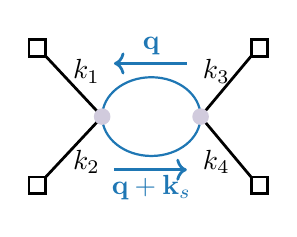
\begin{tikzpicture}[baseline={([yshift=-.5ex]current bounding box.center)}, line width=1. pt, scale=2.5]
    \draw[blue3, thick] (0.25,0) ellipse (0.25 and 0.20);
    \draw[black] (0, 0) -- (-0.285, 0.305);
    \draw[black] (0, 0) -- (-0.285, -0.305);
    \node[draw, rectangle, minimum width=6.0pt, minimum height=6.0pt, inner sep=0pt, anchor=south east] at (-0.28,0.3) {};
    \node[draw, rectangle, minimum width=6.0pt, minimum height=6.0pt, inner sep=0pt, anchor=north east] at (-0.28,-0.3) {};
    \draw[black] (0.5, 0) -- (0.755, 0.305);
    \draw[black] (0.5, 0) -- (0.755, -0.305);
    \draw[draw=lightgray2, fill=lightgray2] (0, 0) circle (.035cm);
    \draw[draw=lightgray2, fill=lightgray2] (0.5, 0) circle (.035cm);
    \node[draw, rectangle, minimum width=6.0pt, minimum height=6.0pt, inner sep=0pt, anchor=south west] at (0.75,0.3) {};
    \node[draw, rectangle, minimum width=6.0pt, minimum height=6.0pt, inner sep=0pt, anchor=north west] at (0.75,-0.3) {};
    \node at (-0.08, 0.23) {$k_1$};
    \node at (-0.08, -0.23) {$k_2$};
    \node at (0.58, 0.23) {$k_3$};
    \node at (0.58, -0.23) {$k_4$};
    \node at (0.25,0.36){\textcolor{blue3}{$\mb q$}};
    \node at (0.25,-0.36){\textcolor{blue3}{$\mb q+\mb k_s$}};
    \draw[<-,blue3] (0.06,0.27)--(0.43,0.27);
    \draw[->,blue3] (0.06,-0.27)--(0.43,-0.27);
\end{tikzpicture}
    \caption{SK diagrams for four-point correlators with bubble topology. The external lines represent conformally coupled scalars, while the blue loop lines represent massive scalars. The \(\Box\) vertices lie on the future boundary, and the \textcolor{lightgray2}{$\bullet$} vertices denote bulk insertions on the two Schwinger-Keldysh contours, with \(+\) and \(-\) corresponding to the time-ordered and anti-time-ordered branches, respectively. Contributions from all SK branches are summed.\label{fig_bubble}}
\end{figure}

The main technical difficulty lies in the four bulk-to-bulk propagators,
\begin{align}
G_{-+}(k;\tau_1,\tau_2)\equiv&~u(k,\tau_1)u^*(k,\tau_2)\,, \notag\\
G_{+-}(k;\tau_1,\tau_2)\equiv&~u^*(k,\tau_1)u(k,\tau_2)\,, \notag\\
G_{\pm\pm}(k;\tau_1,\tau_2)=&~\theta_{12}G_{\mp\pm}(k;\tau_1,\tau_2)
+\theta_{21}G_{\pm\mp}(k;\tau_1,\tau_2)\,,
\label{eq:proptype}
\end{align}
where the mode function and its complex conjugate are
\begin{align}
u(k,\tau)&=\frac{\sqrt\pi}{2}e^{\ii\pi \nu/2}(-\tau)^{d/2}\mathrm H_{\nu}^{(1)}(-k\tau)\,, \notag\\
u^*(k,\tau)&=\frac{\sqrt\pi}{2}e^{-\ii\pi \nu^*/2}(-\tau)^{d/2}\mathrm H_{\nu^*}^{(2)}(-k\tau)\,.
\end{align}
Here \(\nu\equiv\sqrt{d^2/4-m^2}\) is the mass parameter. For notational simplicity, we focus on the complementary-series case in which \(\nu\) is real, while our method applies equally well to the principal-series case where \(\nu\) is purely imaginary. We also use the shorthand \(\theta_{ij}\equiv\theta(\tau_i-\tau_j)\). By contrast, the bulk-to-boundary propagators of \(\phi\) take the simple form
\begin{align}
K_\pm(k;\tau)= \frac{\tau}{2k}e^{\pm \ii k\tau}\,.
\end{align}
In particular, up to trivial prefactors, the product of all bulk-to-boundary propagators attached to a given vertex depends only on the total energy \(P\) flowing into that vertex,
\begin{align}
\prod_i K_\pm(k_i;\tau)\propto e^{\pm \ii P\tau}\,,\qquad
P\equiv \sum_i k_i\,.
\end{align}

We denote by \(\mathcal T_{\mathsf a\mathsf b}\), with \(\mathsf a,\mathsf b\in\{+,-\}\), the contribution from the SK branch in which the vertices at \(\tau_1\) and \(\tau_2\) lie on the \(\mathsf a\) and \(\mathsf b\) contours, respectively. Of the four branches, \(\mathcal T_{++}\) and \(\mathcal T_{--}\) are more involved because \(G_{++}\) and \(G_{--}\) each contain both \(\theta_{12}\) and \(\theta_{21}\) terms. Since \(\mathcal T_{++}=\mathcal T_{--}^*\), it suffices to consider \(\mathcal T_{--}\). For the simplest contact interaction \(a^{d+1}\phi^2\sigma^2\), one finds
\begin{align}\label{eq_Feynmanrule}
\mathcal T_{--} \propto&~ \int_{-\infty}^0 \frac{\di \tau_1}{(-\tau_1)^{d+1}}\frac{\di \tau_2}{(-\tau_2)^{d+1}} \notag\\
&\times K_-(k_1;\tau_1)K_-(k_2;\tau_1)K_-(k_3;\tau_2)K_-(k_4;\tau_2) \notag\\
&\times \int \frac{\di^d\mb q}{(2\pi)^d}\,G_{--}(|\mb q|;\tau_1,\tau_2)G_{--}(|\mb q+\mb k_s|;\tau_1,\tau_2)\,.
\end{align}
This motivates the following integral family for the bubble topology, which accommodates vertices with arbitrary numbers of derivatives:
\begin{widetext}
\ie\label{eq_Idef2}
&I[\{\bm n\},\{a_1,a_2\},\{b_1,b_2\}]
=\int \frac{\di^d \mb q}{(2\pi)^d}
\frac{1}{|\mb q|^{b_1}|\mb k_s+\mb q|^{b_2}} I^{\tau}_{\bm n} \,,\quad\quad I^{\tau}_{\bm n} \equiv \int_{-\infty}^0 \di\tau_1\di\tau_2\,\hat{I}^{\tau}_{\bm n} \,, \n \\
& \hat{I}^{\tau}_{\bm n}=e^{-\ii P_1\tau_1 - \ii P_2 \tau_2}\,(-\tau_1)^{a_1}(-\tau_2)^{a_2} \left[ \theta_{21}h_{n_1}^{(1)}(-|\mb q|\tau_1)h_{n_2}^{(2)}(-|\mb q|\tau_2)
+\theta_{12}h_{n_1}^{(2)}(-|\mb q|\tau_1)h_{n_2}^{(1)}(-|\mb q|\tau_2)\right] \\
&~~~~~~~~~~~~~\times \left[\theta_{21}h_{n_3}^{(1)}(-|\mb q+\mb k_s|\tau_1)h_{n_4}^{(2)}(-|\mb q+\mb k_s|\tau_2)
+\theta_{12}h_{n_3}^{(2)}(-|\mb q+\mb k_s|\tau_1)h_{n_4}^{(1)}(-|\mb q+\mb k_s|\tau_2)\right]\,. 
\fe
\end{widetext}

Here \(P_1=k_1+k_2\) and \(P_2=k_3+k_4\) are the energies flowing into the two vertices. Equation~\eqref{eq:hdef} implies that any \(h_n^{(\alpha)}(z)\) with \(n\ge 2\) can be recursively reduced to a linear combination of \(h_{0}^{(\alpha)}(z)\) and \(h_{1}^{(\alpha)}(z)\). It is thus sufficient to restrict all indices \(n_i\) to \(\{0,1\}\). The contribution in \eqref{eq_Feynmanrule} then corresponds, up to an overall normalization, to
\begin{equation}\label{eq_TinI}
\mathcal T_{--} \propto I[\{0,0,0,0\},\{1+2\nu,1+2\nu\},\{-2\nu,-2\nu\}]\,.
\end{equation}

The family \eqref{eq_Idef2} is manifestly closed under IBP identities generated by total derivatives in the loop momentum \(\mb q\). Temporal IBP is more subtle, because derivatives acting on \(\theta_{21}\) and \(\theta_{12}\) generate contact terms proportional to \(\delta(\tau_1-\tau_2)\). As explained in Ref.~\cite{Chen:2023iix}, after using this delta function to localize one of the time integrals, the collapsed propagator is evaluated through the Wronskian relation
\begin{align}
h_{n_1}^{(1)}(z)\,h_{n_2}^{(2)}(z)-h_{n_1}^{(2)}(z)\,h_{n_2}^{(1)}(z)
= (n_1-n_2)\frac{4\ii}{\pi}z^{-2\nu-1}\,,
\label{eq_propcontract}
\end{align}
with \(n_{1,2}\in\{0,1\}\). It follows that, under \(\di\tau\)-IBP, the family \eqref{eq_Idef2} closes up to residual terms belonging to the tadpole-like family 
\begin{widetext}
\begin{align}\label{eq_Rdef}
&~R[\{n_1,n_2\},\{a\},\{b_1,b_2\}]
\equiv\int_{-\infty}^0 \di\tau \int \frac{\di^d \mb q}{(2\pi)^d}  \frac{e^{-\ii P_0\tau} (-\tau)^{a}}{|\mb q|^{b_1}|\mb k_s+\mb q|^{b_2}}  \frac{1}{2}\sum_{i=0,1} h_{n_1}^{(1+i)}(-|\mb q|\tau)h_{n_2}^{(2-i)}(-|\mb q|\tau) %+h_{n_1}^{(2)}(-|\mb q|\tau)h_{n_2}^{(1)}(-|\mb q|\tau) 
\end{align}
\end{widetext}
where \(P_0\equiv P_1+P_2\). When \(b_2=0\), \(R\) reduces to the standard tadpole family.

For comparison, \(\mathcal T_{-+}\), in which the first bulk vertex lies on the \(+\) contour and the second on the \(-\) contour, is naturally encoded in the family
\ie\label{eq_Ipmdef}
& \widetilde I[\{\bm{n}\},\{a_1,a_2\},\{b_1,b_2\}] = \int_{-\infty}^0 \di\tau_1\di\tau_2 \int \frac{\di^d \mb q}{(2\pi)^d}\,\\
&\times  e^{-\ii P_1\tau_1+\ii P_2 \tau_2}\,
	\frac{(-\tau_1)^{a_1}(-\tau_2)^{a_2}}{|\mb q|^{b_1}|\mb k_s+\mb q|^{b_2}} h_{n_1}^{(1)}(-|\mb q|\tau_1)h_{n_2}^{(2)}(-|\mb q|\tau_2) \\
&\times h_{n_3}^{(1)}(-|\mb q+\mb k_s|\tau_1)h_{n_4}^{(2)}(-|\mb q+\mb k_s|\tau_2)\,.
\fe
Similar to \eqref{eq_TinI}, we have
\begin{equation}
\mathcal T_{-+} \propto \widetilde I[\{0,0,0,0\},\{1+2\nu,1+2\nu\},\{-2\nu,-2\nu\}]\,.
\end{equation}
Since \eqref{eq_Ipmdef} contains no step functions, it closes under both \(\di q\)-IBP and \(\di\tau\)-IBP, with no additional tadpole-like family. Its IBP relations follow from those of \eqref{eq_Idef2} upon replacing \(P_2\to -P_2\) and discarding all terms proportional to \(R\). We therefore restrict attention to the family \eqref{eq_Idef2}. The complete IBP relations are given in the Supplemental Material. The top-sector relations of \eqref{eq_Idef2} immediately reveal the following conserved \emph{odevities}:
\begin{enumerate}
\item For both \(\di q\)-IBP and \(\di \tau\)-IBP, the odevities of \(n_1+n_2+b_1\) and \(n_3+n_4+b_2\) are conserved. Each conserved parity is naturally associated with one propagator.
\item For \(\di q\)-IBP, the odevities of \(n_1+n_3+a_1\) and \(n_2+n_4+a_2\) are also conserved \footnote{Since our reduction combines \(\di q\)-IBP and \(\di \tau\)-IBP, this second pair will not be used below.}.
\end{enumerate}
In particular, in the residual family \(R\) defined in \eqref{eq_Rdef}, the line carrying momentum \(\mb k_s+\mb q\) no longer contains any Hankel functions, so the corresponding conserved parity is simply the parity of \(b_2\).

More generally, the first conservation pattern extends straightforwardly to \(n\)-propagator families, yielding \(2^n\) IBP-closed subsystems and thus significantly simplifying the reduction of dS loop integrals. For the bubble family considered here, we restrict attention to the even-even subsystem,
\begin{align}
n_1+n_2+b_1 \ \text{even}\,,\qquad n_3+n_4+b_2 \ \text{even}\,.
\label{eq:parity_even_sector}
\end{align}
We reduce this subsystem using the user-defined-system module of Kira \cite{Maierhofer:2017gsa,Klappert:2020nbg,Lange:2025fba}. It contains 14 top-sector master integrals and 5 in the remaining-term family.

\section{\(\di\log\) integrands of the top sector and the alphabet}
\label{sec:baikov}

In this section, we construct the \(\di\log\)-form integrands for the top sector and determine the alphabet of the associated differential system. Since the Baikov representation is particularly well suited to the construction of \(\di\log\)-forms in flat spacetime, we first adapt it to cosmological correlators and then explain how a viewpoint inspired by fibration intersection theory motivates our construction.

For the dS bubble diagram, we introduce the Baikov variables \cite{Baikov:1996iu}
\begin{align}
x_1=\sqrt{z_1}=|\mb q|\,,\qquad x_2=\sqrt{z_2}=|\mb q+\mb k_s|\,.
\end{align}
Using the same change of variables as in the flat-space Baikov representation, one finds the normalized measure
\ie
&\frac{2}{\pi^{d/2}}\,\di^d q
= C_d\,\mG^{\frac{d-3}{2}}\mK^{-\frac{d-2}{2}}\,\di z_1\,\di z_2\,,\ 
C_{d} = \frac{\pi^{-1/2}}{\Gamma[(d-1)/2]}\,, \\
&\mK=k_s^2\,, \ 
\mG=\frac{1}{4}\Big(2 z_1 k_s^2+2 z_2 k_s^2-k_s^4-z_1^2-z_2^2+2 z_1 z_2\Big)\,,
\fe
valid for general spatial dimension \(d\). For later use, note that \(\di z_i=2x_i\,\di x_i\), so that a factor \(x_i^{-b_i}\) in the \(z_i\) representation is shifted by one power when rewritten in terms of \(x_i\):
\begin{align}
&~I[\{\bm{n}\},\{a_1,a_2\},\{b_1,b_2\}]
\sim
\int \cdots \times \frac{\di z_1}{x_1^{b_1}}\frac{\di z_2}{x_2^{b_2}}\n\\
=&~
\int \cdots \times 4\,\frac{\di x_1}{x_1^{b_1-1}}\frac{\di x_2}{x_2^{b_2-1}}\,.
\end{align}
The Baikov representation also allows the dimensional recurrence relations \cite{Tarasov:1996br,Lee:2010wea} to be carried over from flat spacetime to dS space; the relevant relation is given in \eqref{shift}.

Since IBP shifts the indices \(a_i\) and \(b_i\) only by integers, it is convenient to absorb the common \(\nu\)-dependent offsets into the index notation and rewrite
\begin{align}
	&I[\{\bm{n}\},\{a_0+a_1',a_0+a_2'\},\{b_0+b_1',b_0+b_2'\}]\notag\\
	\to &I[\{\bm{n}\},\{a_1',a_2'\},\{b_1',b_2'\}]
\end{align}
where, as seen from \eqref{eq_TinI}, these shifts are
\begin{align}
	a_0 = 2\nu  \,, \quad b_0= -2\nu \,.
\end{align}

%在平直时空中，Baikov表示的被积函数可以写作$u \phi$,对于多项式型被积函数，$u=\prod_i P_i^{\beta_i}$的情况, twisted connection $\omega\equiv\di u/u=\prod_i \beta_i \di\log P_i$ 天然的是$\di\log$-form, 而此时若构造一些列$\di\log$-form的$\phi$为主积分，利用$\omega$与$\phi$是$\di\log$-form的性质，可以证明其满足$\di\log$-form的微分方程。
We now briefly recall the relevant aspect of intersection theory. In flat spacetime, a Baikov integrand can be written as \(u\,\phi\), with \(u=\prod_i P_i^{\beta_i}\), for example \(u=\mG^{-\ep}\), so that the integrand is built entirely from polynomial factors. The associated twisted connection,
\begin{align}
\omega \equiv \frac{\di u}{u}=\sum_i \beta_i\,\di\log P_i\,,
\end{align}
is therefore naturally of \(\di\log\)-form. It was further proved by intersection theory in \cite{Chen:2023kgw,Chen:2024ovh} that, \(\di\log\)-form  master integrands \(\{\phi_i\}\) with \(\di\log\)-form $\omega$ will give  \(\di\log\)-form differential equations.
%在过去一般认为Intersection theory只能用于这种多变量型的被积函数，而本文中遇到的dS时空的被积函数中含有Hankel函数。我们创新性的把fibration Intersection theory的中间步骤重新理解为了一种新的Intersection theory的形式，可作用于$\Phi.\U$ 其中$U$是积分核函数族的一组主积分，$Phi$则是一组含有被积函数的系数。而dS时空的圈积分中，$\tau$积分部分可以作为积分核U. 但是需要注意，此时不同于平直时空，$\di U=\Omega.U$中的twisted connection $\Omega$是积分核的主积分U的微分方程，并不天然的是$\di\log$形式。 我们猜想，当我们选取U使得$\Omega$是$\di\log$形式并构造$\Phi$是$\di\log$形式作为完整函数族的主积分时时，自动可以使得其满足的微分方程是$\di\log$形式。

Intersection theory is usually formulated for polynomial-type integrands, whereas the dS integrands relevant here involve Hankel functions. To address this, we reinterpret the intermediate step in the fibration approach to intersection theory \cite{Frellesvig:2019uqt} as suggesting a generalized intersection-theoretic structure acting on objects of the form \(\Phi\cdot\mathbf U\). Here \(\mathbf U\) denotes a vector of master integrals for a kernel family, while \(\Phi\) collects the remaining part of the integrand. Unlike in the standard setting, we do not ask the integrand defining \(\mathbf U\) to be polynomial type.

For dS loop integrals, the \(\tau\) integral can be incorporated into the kernel \(\mathbf U\). Unlike in flat spacetime, the twisted connection \(\Omega\), defined by
\begin{align}
\di \mathbf U=\Omega\cdot\mathbf U\,,
\end{align}
encodes the differential equations satisfied by the kernel integrals and is not automatically \(\di\log\)-form. We conjecture that, if \(\mathbf U\) is chosen such that \(\Omega\) is  \(\di\log\)-form and \(\{\Phi\}\) of master integrals are simultaneously chosen to be \(\di\log\)-form, then the corresponding differential equations automatically take \(\di\log\)-form. We implement this idea below.

We choose the kernel to be
\begin{align}
	\mathbf{U} = x_1^{-b_0}x_2^{-b_0}\,\mG^{-\ep}\mK^{\ep}\,I^{\tau}_{\bm n}\,,
\end{align}
where \(\ep\) is the dimensional regulator, \(d=3-2\ep\), the one-loop Baikov measure contributes the factor \(\mG^{-\ep}\mK^{\ep}\), and \(I^{\tau}_{\bm n}\) with all $n_i$  running over 0 and 1 denotes the master integrals of the \(\tau\)-integral family, as studied in \cite{Chen:2023iix}. 
%\ie
%&I^{\tau}_{\bm n}(x_1,x_2;P_1,P_2)\equiv \int_{-\infty}^0 \di\tau_1\di\tau_2\,\hat{I}^{\tau}_{\bm n}\,, \\
%&\hat{I}^{\tau}_{\bm n} \equiv  e^{-\ii P_1\tau_1-\ii P_2\tau_2}\,(-\tau_1)^{a_0}(-\tau_2)^{a_0} \\
%	&~~~~~~\times \left[ \theta_{21}h_{n_1}^{(1)}(-x_1\tau_1)h_{n_2}^{(2)}(-x_1\tau_2) h_{n_3}^{(1)}(-x_2\tau_1)h_{n_4}^{(2)}(-x_2\tau_2)\, \right. \\
% &\left. ~~~~~~ + \theta_{12} h_{n_1}^{(2)}(-x_1\tau_1)h_{n_2}^{(1)}(-x_1\tau_2) h_{n_3}^{(2)}(-x_2\tau_1)h_{n_4}^{(1)}(-x_2\tau_2) \right]\,
%\fe
\cite{Chen:2023iix} also tells that the differential equations of $I^{\tau}_{\bm n}$ take the \(\di\log\)-form 
\begin{align}
	\di I^{\tau}_{\bm m}=(\di\Omega_{\bm m\bm n}^{\tau})\,I^{\tau}_{\bm n} \,, \quad \di\Omega^{\tau}=\di\Omega_{x_1}+\di\Omega_{x_2}+\di\Omega_{ex}\,,  \label{eq:Omegatau}
\end{align}
where the one-forms in \(\di\Omega^{\tau}\) are built from \(\di\log x_1\), \(\di\log x_2\), and \(\di\log(P_i\pm x_1\pm x_2)\), and the three contributions are denoted by \(\di\Omega_{x_1}\), \(\di\Omega_{x_2}\), and \(\di\Omega_{ex}\), respectively. The explicit top-sector expressions can be found in the ancillary file \zq{file}.
 %\cjq{哪呢？引下公式？}
Accordingly, the twisted connection associated with \(\mathbf{U}\) is also of \(\di\log\)-form,
\begin{align}
	\di \mathbf{U}=&(\di \Omega)\cdot \mathbf{U}\notag\\
 =&\Big(\di\Omega^{\tau}-b_0(\di\log x_1+\di\log x_2)\notag\\
 &~~~~~~~~~~~~~~~~~-\ep(\di\log \mG-\di\log \mK)\Big)\cdot \mathbf{U} \,.
\end{align}

To construct \(\di\log\)-form choices of \(\Phi\), we first note the following useful building blocks:
\begin{align}
	\di\log z_1&=2\di\log x_1\, ,\notag\\
	\frac{\sqrt{z_2 k_s^2}\,\di z_1}{\mG}
	&= - \di\log \left(\frac{2 \sqrt{z_2 k_s^2}+k_s^2-z_1+z_2}{-2 \sqrt{z_2 k_s^2}+k_s^2-z_1+z_2}\right)
\end{align}
and $(z_1\leftrightarrow z_2)$. The connection \(\Omega^\tau\) contains additional \(\di\log\)-type building blocks. However, some of them involve denominators of the form \(P_i \pm x_1 \pm x_2\), and using such factors directly would enlarge the integral family. To avoid this, we only use combinations that can be rewritten back in terms of the original family:
\begin{align}
	&\partial_{P_j}\Omega_{ex}\,\di x_i = \partial_{P_j}\Omega^{\tau}\,\di x_i 
 %= - \ii \tau_i \, \di x_i 
 \, , \n\\
	&\partial_{x_j}\Omega_{ex}\,\di x_i = (\partial_{x_j}\Omega^{\tau}-\partial_{x_j}\Omega_{x_j})\,\di x_i \,,
\end{align}
Indeed, \(\partial_{P_j}\Omega^{\tau}\) is harmless because, when acting on \(I^{\tau}_{\bm n}\), it is equivalent to differentiating the kernel with respect to \(P_j\), which simply inserts a factor of \(-\ii\tau_j\). Likewise, \(\partial_{x_j}\Omega^{\tau}\) can be related to \(\di I^{\tau}_{\bm n}\) and then handled by further IBP reduction, while \(\partial_{x_j}\Omega_{x_j}\) involves only \(1/x_j\) and therefore does not introduce any new denominator structure.

Using these building blocks, we choose the following \(\di\log\)-form integrals as master integrals:
\paragraph{For $\Phi=\delta_{\bm n\bm m}\,\frac{\sqrt{z_2 k_s^2}\,\di z_1}{\mG}\frac{\di z_2}{z_2}$}
\begin{align}
	&I[\{0, 0, 0, 1\}, \{0, 0\}, \{0, 1\}, d=1]\,,\notag\\
 &I[\{1, 1, 0, 1\}, \{0, 0\}, \{0, 1\}, d=1]\,.
 \end{align}
\paragraph{For $\Phi=\delta_{\bm n\bm m}\,\frac{\sqrt{z_2 k_s^2}\,\di z_1}{\mG}\,\tau_2\,\di x_2$}
\begin{align}
	& I[\{0, 0, 0, 0\}, \{0, 1\}, \{0, 0\}, d=1]\,, \notag\\
 &I[\{0, 0, 1, 1\}, \{0, 1\}, \{0, 0\}, d=1]\,,\notag\\
 &I[\{1, 1, 1, 1\}, \{0, 1\}, \{0, 0\}, d=1]\,.
\end{align}
\paragraph{For $\Phi=\delta_{\bm n\bm m}\,\tau_2\,\di x_1\,\frac{\di x_2}{x_2}$}
\begin{align}
	& k_sI[\{0, 1, 0, 0\}, \{0, 1\}, \{1, 2\}, d=3]\,, \notag\\
	&k_sI[\{0, 1, 1, 1\}, \{0, 1\}, \{1, 2\}, d=3]\,, \nonumber\\
	& k_sI[\{1, 0, 0, 0\}, \{0, 1\}, \{1, 2\}, d=3]\,, \notag\\
	&k_sI[\{1, 0, 1, 1\}, \{0, 1\}, \{1, 2\}, d=3]\,.
\end{align}
\paragraph{For $\Phi=\delta_{\bm n\bm m}\,\frac{\di x_1\,\di x_2}{x_1 x_2}$}
\begin{align}
	& k_sI[\{0, 0, 0, 0\}, \{0, 0\}, \{2, 2\}, d=3]\,, \notag\\
	&k_sI[\{0, 0, 1, 1\}, \{0, 0\}, \{2, 2\}, d=3]\,, \notag\\
 & k_sI[\{1, 1, 1, 1\}, \{0, 0\}, \{2, 2\}, d=3]\,.
\end{align}
\paragraph{For $\Phi=(\partial_{x_2}\Omega_{ex})_{\bm n \bm m}\,\di x_1\,\frac{\di x_2}{x_2}$}
\begin{align}
	& (2 + b_0 + 2\nu)\,I[\{0, 1, 0, 1\}, \{0, 0\}, \{1, 3\}, d=3]\,, \nonumber\\
	& (2 + b_0 + 2\nu)\,I[\{0, 1, 1, 0\}, \{0, 0\}, \{1, 3\}, d=3]\,.
\end{align}
For each choice of \(\bm m\), the combination \(\int \Phi_{\bm m\bm n}U_{\bm n}\) defines a \(\di\log\) integral. Using symmetry relations together with the parity constraints, we select from all possible \(\bm m\) the independent master integrals belonging to the even-even subsystem. Since rewriting \(\Phi\) in the original integral representation may involve integrals in \(d=1-2\ep\), we indicate the dimension explicitly for each master integral. In subsequent calculations, these can first be shifted back to \(d=3\) by the flat-space dimensional shift formula \eqref{shift}, after which the IBP reduction can be carried out uniformly.





The differential equations for the resulting master-integral basis are verified to be of \(\di\log\)-form. The corresponding alphabet is
\begin{widetext}
\begin{align}
	\mathcal{A} = \left\{ x, x\pm 1, x\pm \sqrt{1+2\epsilon}, x \pm \frac{1+2\nu}{\sqrt{2}} \pm \frac{ \sqrt{3+4\epsilon+4\nu(1+\nu)}}{\sqrt{2}} \right\}\,.
\end{align}
\end{widetext}
with \(x=P_1/k_s=P_2/k_s\).
The coefficient matrices are given in \cjq{attachment or github link?}. We note that both the alphabet and the coefficient matrices involve square roots depending on \(\epsilon\) and \(\nu\), such as \(\sqrt{1+2\epsilon}\) and \(\sqrt{3+4\epsilon+4\nu(1+\nu)}\). This differs from polynomial-type integrands in flat spacetime, where the \(\di\log\)-form typically involves only kinematic variables and the coefficients are rational functions of the power parameters \(\beta_i\) in \(u=\prod_i P_i^{\beta_i}\), for example \(\ep\). Understanding this difference would be interesting to pursue further.






\section{Conclusion}
In this letter, we studied the IBP reduction and differential equations of 1-loop bubble diagram in dS space. We first indicate the parity property of dS loop IBP system, which could scale down the size of the n propagators IBP-system by a factor of $2^n$, which significantly enhances the feasibility of this computational approach. We successful apply the IBP reduction and the differential equations method to loop massive cosmological correlators. This demonstrates the viability of them as a systematic and automated framework for perturbative field theory calculations in dS space.
 We also explore the interesting mathematic property of this system. We indicate the fibration intersection theory could be generalized to the cases that $\bm{\rm U}$ is not polynomial-type. Based on that, we conjecture that select $\di\log$-form twist connection and construct $\di\log$-form $\Phi$ as master integrals could directly give $\di\log$-form differential equations. We introduce Baikov representation to dS case and find it helpful for $\di\log$-form $\Phi$ construction. Then the result of the bubble example verify the conjecture and we get a simple alphabet of this system.




\bibliographystyle{apsrev4-1}
\bibliography{letter}
\clearpage
\appendix
\begin{widetext}
\section*{Supplementary Material}
\subsection{Reduction relations for top-sector families}
As mentioned in \cite{Chen:2023iix}, for bubble integral families with $\theta_{12}$ or $\theta_{21}$ present, time IBP relations, which involve total derivatives $\int \pd_{\tau_i}[\cdots]=0$, will collapse one time integration and finally produce tadpole families. In this case, the propagator being collapsed will give the following factor
\bge
h_{n_1}^{(1)}(-k\tau_i)\,h_{n_2}^{(2)}(-k\tau_i) - h_{n_1}^{(2)}(-k\tau_i)\,h_{n_2}^{(1)}(-k\tau_i)
= \delta_{n_1+ n_2,1} (-1)^{n_1+1}e^{ \pi \text{Im}[\nu]} \frac{  4 \ii }{\pi}  (-k\tau_i)^{-2\nu-1} \,.  \label{eq_propcontract_app}
\ede
which, in our integral-family language, is implemented as a shift of the corresponding $|k|$-power index by $2\nu+1$ and the $\tau$-power index by $-2\nu-1$. And in the remaining families, there is only one time integration. These kinds of terms are known as remaining terms \cite{Chen:2023iix}, and will be denoted by $R$.

%In particular, since the $R$ families originate from contracting one propagator in the top sector, the contracted line carries an extra $(-k)^{-2\nu-1}$ factor from the Wronskian. In the Mathematica/Kira implementation we keep the momentum baselines trivial,
%\[
%|q|^{-b_1}\,|\bm k_s+\bm q|^{-b_2},
%\qquad b_{10}=0, \quad b_{20}=-2\nu,
%\]
%and the remaining-term factor is tracked explicitly by the $b$ shifts (e.g. $b_1\to b_1+2\nu+1$) in Eqs.~(\ref{eq:timeIBP_tau1})--(\ref{eq:timeIBP_tau2}).


First, let us consider the time-IBP relations. For $\pd_{\tau_1}$, we have:
\begin{align}
	0 = & - \ii P_1 I[\{n_1,n_2,n_3,n_4\},\{a_1,a_2\},\{b_1,b_2\}] - a_1I[\{n_1,n_2,n_3,n_4\},\{a_1-1,a_2\},\{b_1,b_2\}]\nonumber \\
	    & - I[\{n_1+1,n_2,n_3,n_4\},\{a_1,a_2\},\{b_1-1,b_2\}] - I[\{n_1,n_2,n_3+1,n_4\},\{a_1,a_2\},\{b_1,b_2-1\}]\nonumber      \\
	    & +\delta_{n_1+n_2,1}(-1)^{n_1+1}R_1[\{n_3,n_4\},\{a_1+a_2-2\nu-1\},\{b_1+2\nu+1,b_2\}]\nonumber                \\
	    & +\delta_{n_3+n_4,1}(-1)^{n_3+1}R_2[\{n_1,n_2\},\{a_1+a_2-2\nu-1\},\{b_1,b_2+2\nu+1\}]\,, \label{eq:timeIBP_tau1}
\end{align}
and similarly for $\partial_{\tau_2}$:
\begin{align}
	0 = & - \ii P_2 I[\{n_1,n_2,n_3,n_4\},\{a_1,a_2\},\{b_1,b_2\}] - a_2I[\{n_1,n_2,n_3,n_4\},\{a_1,a_2-1\},\{b_1,b_2\}]\nonumber \\
	    & - I[\{n_1,n_2+1,n_3,n_4\},\{a_1,a_2\},\{b_1-1,b_2\}] - I[\{n_1,n_2,n_3,n_4+1\},\{a_1,a_2\},\{b_1,b_2-1\}]\nonumber      \\
	    & +\delta_{n_1+n_2,1}(-1)^{n_2+1}R_1[\{n_3,n_4\},\{a_1+a_2-2\nu-1\},\{b_1+2\nu+1,b_2\}]\nonumber                \\
	    & +\delta_{n_3+n_4,1}(-1)^{n_4+1}R_2[\{n_1,n_2\},\{a_1+a_2-2\nu-1\},\{b_1,b_2+2\nu+1\}]\,, \label{eq:timeIBP_tau2}
\end{align}
where $\nu$ is the common mass parameter.

As for the momentum-IBP relations, we introduce
\begin{align}
	x_1 \equiv |\bm q|\,,\qquad x_2 \equiv |\bm q+\bm k_s|\,,\qquad
	\mathcal{O}_1 \equiv \bm q^i \pd_{\bm q^i}\,,\qquad
	\mathcal{O}_2 \equiv (\bm q^i+\bm k_s^i)\pd_{\bm q^i}\,,
\end{align}
whose actions on $(x_1,x_2)$ are
\begin{align}
	\mathcal{O}_1 x_1 & = x_1\,, \nonumber\\
	\mathcal{O}_1 x_2 & = \frac{1}{2}x_2^{-1}(x_1^2 + x_2^2 - k_s^2)\,, \nonumber\\
	\mathcal{O}_2 x_1 & = \frac{1}{2}x_1^{-1}(x_1^2 + x_2^2 - k_s^2)\,, \nonumber\\
	\mathcal{O}_2 x_2 & = x_2\,.
\end{align}
Equivalently, for any function $F(x_1,x_2)$ one has the chain rule
\begin{align}
	\mathcal{O}_\alpha F = (\mathcal{O}_\alpha x_1)\,\partial_{x_1}F + (\mathcal{O}_\alpha x_2)\,\partial_{x_2}F\,,\qquad \alpha=1,2\,.
\end{align}

From $\int \pd_{\bm q^i}[\bm q^i \cdots ]=0$ one may write an intermediate step in terms of the composite operator acting on the full integrand,
\begin{align}
	0 &= \int_{-\infty}^0 \di\tau_1\di\tau_2\int \frac{\di^d \bm q}{(2\pi)^d}\,
	\Big[d+\mathcal{O}_1\Big] \nonumber\\ 
	& \Bigg[
	e^{-\ii P_1\tau_1-\ii P_2\tau_2}
	\frac{(-\tau_1)^{a_1}(-\tau_2)^{a_2}}{x_1^{b_1}x_2^{b_2}}\,
	h_{n_1}^{(1)}(-x_1\tau_1)h_{n_2}^{(2)}(-x_1\tau_2) \times h_{n_3}^{(1)}(-x_2\tau_1)h_{n_4}^{(2)}(-x_2\tau_2)\Bigg] \nonumber\\
	& =  \int_{-\infty}^0 \di\tau_1\di\tau_2\int \frac{\di^d \bm q}{(2\pi)^d}\,
	\Bigg[d+(\mathcal{O}_1 x_1)\partial_{x_1} +(\mathcal{O}_1 x_2)\partial_{x_2}\Bigg] \nonumber\\
	&\Bigg[
	e^{-\ii P_1\tau_1-\ii P_2\tau_2}
	\frac{(-\tau_1)^{a_1}(-\tau_2)^{a_2}}{x_1^{b_1}x_2^{b_2}}\,
	h_{n_1}^{(1)}(-x_1\tau_1)h_{n_2}^{(2)}(-x_1\tau_2)
	  \times h_{n_3}^{(1)}(-x_2\tau_1)h_{n_4}^{(2)}(-x_2\tau_2)\Bigg]\,. \label{eq:momIBP_qdot_chainrule}
\end{align}
Expanding the derivatives using $\partial_x x^{-b}=-(b/x)x^{-b}$ and $\partial_x h_n(-x\tau)=(-\tau)\,h_{n+1}(-x\tau)$ yields the closed relation in terms of shifted $I$ integrals:
\begin{align}
	0 =& d\,I[\{n_1,n_2,n_3,n_4\},\{a_1,a_2\},\{b_1,b_2\}] - b_1\,I[\{n_1,n_2,n_3,n_4\},\{a_1,a_2\},\{b_1,b_2\}] \nonumber \\
	&- \frac12 b_2\Big(
	B[\{n_1,n_2,n_3,n_4\},\{a_1,a_2\},\{b_1,b_2\}]  + I[\{n_1,n_2,n_3,n_4\},\{a_1,a_2\},\{b_1-2,b_2+2\}] \nonumber\\
	&-k_s^2\,I[\{n_1,n_2,n_3,n_4\},\{a_1,a_2\},\{b_1,b_2+2\}]
	\Big) +I[\{n_1+1,n_2,n_3,n_4\},\{a_1+1,a_2\},\{b_1-1,b_2\}] \nonumber\\
	&+ I[\{n_1,n_2+1,n_3,n_4\},\{a_1,a_2+1\},\{b_1-1,b_2\}] +\frac12 \Big(
	I[\{n_1,n_2,n_3+1,n_4\},\{a_1+1,a_2\},\{b_1,b_2-1\}] \nonumber\\
	&+ I[\{n_1,n_2,n_3+1,n_4\},\{a_1+1,a_2\},\{b_1-2,b_2+1\}]-k_s^2\,I[\{n_1,n_2,n_3+1,n_4\},\{a_1+1,a_2\},\{b_1,b_2+1\}]
	\Big) \nonumber \\
	&+\frac12\Big(
	I[\{n_1,n_2,n_3,n_4+1\},\{a_1,a_2+1\},\{b_1,b_2-1\}]+ I[\{n_1,n_2,n_3,n_4+1\},\{a_1,a_2+1\},\{b_1-2,b_2+1\}] \nonumber\\
	&-k_s^2\,I[\{n_1,n_2,n_3,n_4+1\},\{a_1,a_2+1\},\{b_1,b_2+1\}]
	\Big)\,,
\label{eq:momIBP_qdot}
\end{align}
where $d$ is the spatial dimension (in dimensional regularization $d=3-2\ep$). The second momentum IBP can be written in the same chain-rule form as
\begin{align}
	0 ={}& \int_{-\infty}^0 \di\tau_1\di\tau_2\int \frac{\di^d \bm q}{(2\pi)^d}\,
	\Big[d+\mathcal{O}_2\Big]\nonumber\\
	&\Bigg[
	e^{-\ii P_1\tau_1-\ii P_2\tau_2}
	\frac{(-\tau_1)^{a_1}(-\tau_2)^{a_2}}{x_1^{b_1}x_2^{b_2}}\,
	h_{n_1}^{(1)}(-x_1\tau_1)h_{n_2}^{(2)}(-x_1\tau_2) \times h_{n_3}^{(1)}(-x_2\tau_1)h_{n_4}^{(2)}(-x_2\tau_2)\Bigg]\,, \label{eq:momIBP_qk_chainrule}
\end{align}
which gives the symmetric relation with the exchanges
\begin{align}
	\{n_1,n_2,n_3,n_4\} &\leftrightarrow \{n_3,n_4,n_1,n_2\}\,, \nonumber\\
	\{b_1,b_2\} &\leftrightarrow \{b_2,b_1\}\,. \nonumber
\end{align}

Note that there is another relation from \eqref{eq:hdef}, called EOM relations:
\begin{align}
	I[\{2,n_2,n_3,n_4\},\{a_1,a_2\},\{b_1,b_2\}] = & - I[\{0,n_2,n_3,n_4\},\{a_1,a_2\},\{b_1,b_2\}]\nonumber      \\
   & - (2\nu+1) I[\{1,n_2,n_3,n_4\},\{a_1-1,a_2\},\{b_1+1,b_2\}]\,, \\
	I[\{n_1,2,n_3,n_4\},\{a_1,a_2\},\{b_1,b_2\}] = & - I[\{n_1,0,n_3,n_4\},\{a_1,a_2\},\{b_1,b_2\}]\nonumber      \\
& - (2\nu+1) I[\{n_1,1,n_3,n_4\},\{a_1,a_2-1\},\{b_1+1,b_2\}]\,, \\
	I[\{n_1,n_2,2,n_4\},\{a_1,a_2\},\{b_1,b_2\}] = & - I[\{n_1,n_2,0,n_4\},\{a_1,a_2\},\{b_1,b_2\}]\nonumber      \\
     & - (2\nu+1) I[\{n_1,n_2,1,n_4\},\{a_1-1,a_2\},\{b_1,b_2+1\}]\,, \\
	I[\{n_1,n_2,n_3,2\},\{a_1,a_2\},\{b_1,b_2\}] = & - I[\{n_1,n_2,n_3,0\},\{a_1,a_2\},\{b_1,b_2\}]\nonumber      \\
     & - (2\nu+1) I[\{n_1,n_2,n_3,1\},\{a_1,a_2-1\},\{b_1,b_2+1\}]\,,
\end{align}
where $\nu$ is the common mass parameter.

In addition to the above IBP relations, we also have some symmetry relations:
\begin{align}
	I[\{n_1,n_2,n_3,n_4\},\{a_1,a_2\},\{b_1,b_2\}] = I[\{n_3,n_4,n_1,n_2\},\{a_1,a_2\},\{b_2,b_1\}]\,.
\end{align}

As our final step, we will show the differential equation of this integral family. Although we set $P_1=P_2$, here we give the $P_1$ and $P_2$-derivative individually:
\begin{align}
	\frac{\partial}{\partial P_1}I[\{n_1,n_2,n_3,n_4\},\{a_1,a_2\},\{b_1,b_2\}] &= \ii\,I[\{n_1,n_2,n_3,n_4\},\{a_1+1,a_2\},\{b_1,b_2\}]\,, \label{eq:GdP1}\\
	\frac{\partial}{\partial P_2}I[\{n_1,n_2,n_3,n_4\},\{a_1,a_2\},\{b_1,b_2\}] &= \ii\,I[\{n_1,n_2,n_3,n_4\},\{a_1,a_2+1\},\{b_1,b_2\}]\,. \label{eq:GdP2}
\end{align}
From
\begin{align}
	\frac{\partial}{\partial k_s}|\bm q+\bm k_s|
	=\frac{k_s^2+\bm k_s\cdot \bm q}{k_s|\bm q+\bm k_s|}
	=\frac{k_s^2+|\bm q+\bm k_s|^2-q^2}{2k_s|\bm q+\bm k_s|}\,,
\end{align}
the $k_s$-derivative gives:
\ie
	&\frac{\partial}{\partial k_s}I[\{n_1,n_2,n_3,n_4\},\{a_1,a_2\},\{b_1,b_2\}] \\
	=&-\frac{b_2}{2k_s}\Big(
	k_s^2\,I[\{n_1,n_2,n_3,n_4\},\{a_1,a_2\},\{b_1,b_2+2\}]
	+I[\{n_1,n_2,n_3,n_4\},\{a_1,a_2\},\{b_1,b_2\}] \\
	&
	-I[\{n_1,n_2,n_3,n_4\},\{a_1,a_2\},\{b_1-2,b_2+2\}]
	\Big)+\frac{1}{2k_s}\Big(
	k_s^2\,I[\{n_1,n_2,n_3+1,n_4\},\{a_1+1,a_2\},\{b_1,b_2+1\}] \\
	&
	+I[\{n_1,n_2,n_3+1,n_4\},\{a_1+1,a_2\},\{b_1,b_2-1\}]
	-I[\{n_1,n_2,n_3+1,n_4\},\{a_1+1,a_2\},\{b_1-2,b_2+1\}]
	\Big) \\
	&+\frac{1}{2k_s}\Big(
	k_s^2\,I[\{n_1,n_2,n_3,n_4+1\},\{a_1,a_2+1\},\{b_1,b_2+1\}]
	+I[\{n_1,n_2,n_3,n_4+1\},\{a_1,a_2+1\},\{b_1,b_2-1\}] \\
	&
	-I[\{n_1,n_2,n_3,n_4+1\},\{a_1,a_2+1\},\{b_1-2,b_2+1\}]
	\Big)\,. \label{eq:Gdks}
\fe

Scaling relation:
\begin{align}
	\left( k_s \frac{\partial}{\partial k_s} + P_1 \frac{\partial}{\partial P_1} + P_2 \frac{\partial}{\partial P_2} \right) I[\{\bm n\},\{a_1,a_2\},\{b_1,b_2\}] \n\\
	= (d - b_1 - b_2 - a_1 - a_2 - 2) I[\{\bm n\},\{a_1,a_2\},\{b_1,b_2\}]\,. \label{eq:Gscaling}
\end{align}

In conclusion, the IBP relations for the top sector are \eqref{eq:timeIBP_tau1}, \eqref{eq:timeIBP_tau2}, \eqref{eq:momIBP_qdot}, and \eqref{eq:momIBP_qk_chainrule} together with the symmetry relations and the EOM relations. The differential equations for the top sector are \eqref{eq:GdP1}, \eqref{eq:GdP2}, and \eqref{eq:Gdks}. The scaling relation \eqref{eq:Gscaling} is used to check our differential equation to be right.




\subsection{Reduction relations for tadpole families $R_1,R_2$}
In the IBP relations of the bubble diagram, there will appear integral families of the tadpole diagram as the remaining terms. Such terms have their own IBP relations. Here we only give the IBP relations for $R_1$, and the corresponding relations for $R_2$ follow via the symmetry $\bm q \to -(\bm q+\bm k_s)$, which exchanges $b_1\leftrightarrow b_2$ and relabels Hankel indices appropriately. The time IBP relation for $R_1$ is
\begin{align}
	0 = & -\ii(P_1+P_2) R_1[\{n_3,n_4\},\{a\},\{b_1,b_2\}] - a R_1[\{n_3,n_4\},\{a-1\},\{b_1,b_2\}] \nonumber       \\
	    & - R_1[\{n_3+1,n_4\},\{a\},\{b_1,b_2-1\}] - R_1[\{n_3,n_4+1\},\{a\},\{b_1,b_2-1\}]\,. \label{eq:R1timeIBP}
\end{align}
and two momentum IBP relations read
\begin{align}
	0 = & d R_1[\{n_3,n_4\},\{a\},\{b_1,b_2\}] - b_1 R_1[\{n_3,n_4\},\{a\},\{b_1,b_2\}] \nonumber                    \\
	    & - \frac12 b_2\Big( R_1[\{n_3,n_4\},\{a\},\{b_1,b_2\}] + R_1[\{n_3,n_4\},\{a\},\{b_1-2,b_2+2\}] -k_s^2 R_1[\{n_3,n_4\},\{a\},\{b_1,b_2+2\}] \Big) \nonumber                                                \\
	    & + \frac12 \Big(
	    R_1[\{n_3+1,n_4\},\{a+1\},\{b_1,b_2-1\}] + R_1[\{n_3+1,n_4\},\{a+1\},\{b_1-2,b_2+1\}] \nonumber\\
	    &-k_s^2 R_1[\{n_3+1,n_4\},\{a+1\},\{b_1,b_2+1\}]
	    \Big)+ \frac12 \Big(
	    R_1[\{n_3,n_4+1\},\{a+1\},\{b_1,b_2-1\}] \nonumber\\
     &+ R_1[\{n_3,n_4+1\},\{a+1\},\{b_1-2,b_2+1\}]-k_s^2 R_1[\{n_3,n_4+1\},\{a+1\},\{b_1,b_2+1\}]
	    \Big)\,. \label{eq:R1momIBP}
    \end{align}
\begin{align}
	0 = & d R_1[\{n_3,n_4\},\{a\},\{b_1,b_2\}] - b_2 R_1[\{n_3,n_4\},\{a\},\{b_1,b_2\}] \nonumber                    \\
	    & - \frac12 b_1\Big( R_1[\{n_3,n_4\},\{a\},\{b_1,b_2\}] + R_1[\{n_3,n_4\},\{a\},\{b_1+2,b_2-2\}] \nonumber     \\
	    & -k_s^2 R_1[\{n_3,n_4\},\{a\},\{b_1+2,b_2\}] \Big)+ R_1[\{n_3+1,n_4\},\{a+1\},\{b_1,b_2-1\}] \\
     &+ R_1[\{n_3,n_4+1\},\{a+1\},\{b_1,b_2-1\}]\,. \label{eq:R1momIBP2}
\end{align}
These two relations come from $\int \pd_{\bm q^i}[\bm q^i\cdots]=0$ and $\int \pd_{\bm q^i}[(\bm q^i+\bm k_s^i)\cdots]=0$ respectively.

Note that in the tadpole case, we also have the relations come from \eqref{eq:hdef}:
\begin{align}
	R_1[\{2,n_4\},\{a\},\{b_1,b_2\}] = & - R_1[\{0,n_4\},\{a\},\{b_1,b_2\}] \nonumber                            \\
 & - (2\nu+1) R_1[\{1,n_4\},\{a-1\},\{b_1,b_2+1\}]\,, \label{eq:R1eom1} \\
	R_1[\{n_3,2\},\{a\},\{b_1,b_2\}] = & - R_1[\{n_3,0\},\{a\},\{b_1,b_2\}] \nonumber                            \\
& - (2\nu+1) R_1[\{n_3,1\},\{a-1\},\{b_1,b_2+1\}]\,. \label{eq:R1eom2}
\end{align}
and the following symmetry relation
\begin{align}
	 R_1[\{n_3,n_4\},\{a\},\{b_1,b_2\}] = R_1[\{n_4,n_3\},\{a\},\{b_1,b_2\}] \label{eq:R1sym}\,. 
\end{align}

Let us turn to the differential equations. take $P_1=P_2=P_0$, the $P_0$-derivative gives:
\begin{align}
	\frac{\partial}{\partial P_0} R_1[\{n_3,n_4\},\{a\},\{b_1,b_2\}] = 2 \ii R_1[\{n_3,n_4\},\{a+1\},\{b_1,b_2\}]\,. \label{eq:R1dP0}
\end{align}
and the $k_s$-derivative gives
\begin{align}
	&\frac{\partial}{\partial k_s} R_1[\{n_3,n_4\},\{a\},\{b_1,b_2\}] \n\\
	=&-\frac{b_2}{2k_s}\Big(
	k_s^2\,R_1[\{n_3,n_4\},\{a\},\{b_1,b_2+2\}] 
	+R_1[\{n_3,n_4\},\{a\},\{b_1,b_2\}] 
	-R_1[\{n_3,n_4\},\{a\},\{b_1-2,b_2+2\}]
	\Big) \nonumber\\
	&+\frac{1}{2k_s}\Big(
	k_s^2\,R_1[\{n_3+1,n_4\},\{a+1\},\{b_1,b_2+1\}] 
	+R_1[\{n_3+1,n_4\},\{a+1\},\{b_1,b_2-1\}] \nonumber\\
	&
	-R_1[\{n_3+1,n_4\},\{a+1\},\{b_1-2,b_2+1\}]
	\Big)+\frac{1}{2k_s}\Big(
	k_s^2\,R_1[\{n_3,n_4+1\},\{a+1\},\{b_1,b_2+1\}] 
	\nonumber\\
 &+R_1[\{n_3,n_4+1\},\{a+1\},\{b_1,b_2-1\}] 
	-R_1[\{n_3,n_4+1\},\{a+1\},\{b_1-2,b_2+1\}]
	\Big)\,. \label{eq:R1dks}
\end{align}

Similarly to the bubble case, we have the following scaling relation:
\begin{align}
	\left( k_s \frac{\partial}{\partial k_s} + P_0 \frac{\partial}{\partial P_0} \right) R_1[\{n_3,n_4\},\{a\},\{b_1,b_2\}] = (d - b_1 - b_2 - a - 1) R_1[\{n_3,n_4\},\{a\},\{b_1,b_2\}]\,, \label{eq:R1scaling}
\end{align}
which will be used to verify the correctness of differential equations.

In conclusion, the IBP relations for remaining terms are \eqref{eq:R1timeIBP}, \eqref{eq:R1momIBP}, and \eqref{eq:R1momIBP2} together with symmetry relations and EOM relations. The differential equations are \eqref{eq:R1dP0} and \eqref{eq:R1dks}. As before, for the remaining terms, we still have a scaling relation \eqref{eq:R1scaling}.

\begin{comment}
Using 
\begin{align}
	\hat{I}[\{\bm{n}\},\{a_1+1,a_2\},\{b_1,b_2\}]
	&=\partial_{P_1}\hat{I}[\{\bm{n}\},\{a_1,a_2\},\{b_1,b_2\}]
	=\left(\partial_{P_1}\Omega_{\bm n\bm m}\right) \,\n\\
	&\times \hat{I}[\{\bm{m}\},\{a_1,a_2\},\{b_1,b_2\}], \n\\
	\hat{I}[\{\bm{n}\},\{a_1,a_2\},\{b_1,b_2\}]
	&=\frac{1}{b_0+b_1-1}\left(\partial_{x_1}\Omega_{\bm n\bm m}\right)\,\n\\
	&\times \hat{I}[\{\bm{m}\},\{a_1,a_2\},\{b_1-1,b_2\}],
\end{align}
one may view $\partial_{P_j}\Omega\,\di x_i\sim \tau_j\,\di x_i$ and
$\partial_{x_j}\Omega\,\di x_i\sim \frac{b_0+b_j-1}{x_j}\di x_i$
as additional $\di\log$-type building blocks at the integrand level. And $\partial_{x_j}\Omega_{x_j}$ will not give the factor $\frac{1}{P_i\pm x_1\pm x_2}$, therefore the effect of such a term is just to modify the coefficients of $\frac{1}{x_j}\di x_i$ in $\partial_{x_j}\Omega\,\di x_i$. The $\di\log$ integrands can be constructed using these building blocks. 
\end{comment}

\subsection{Raising $d=1$ back to $d=3$}
In this section, we demonstrate that all dimension-1 master integrals can be raised to their corresponding dimension-3 master integrals. Therefore, they do not require special treatment in the differential equations. 

For the normalized Baikov measure, one has
\begin{align}
	\frac{2}{\pi^{d/2}}\,\di^d q = C_d\,\mG^{\frac{d-3}{2}}\mK^{-\frac{d-2}{2}}\,\di z_1\,\di z_2\,.
\end{align}
In particular, for $d=1-2\ep$ and $d=3-2\ep$,
\begin{align}\label{shift}
	C_{1-2\ep}\,\mG^{-\ep-1}\mK^{\ep+1/2}
	= \partial_{q^2}\!\left[C_{3-2\ep}\,\mK^{-1/2+\ep}\mG^{-\ep}\right]\,,
\end{align}
where $\partial_{q^2}\equiv\partial_{z_1}+\partial_{z_2}$ and we used $\partial_{q^2}\mG=\mK$ together with $\Gamma(1-\ep)=-\ep\,\Gamma(-\ep)$.

Therefore, for
\begin{align}
	\hat{I}[\{\bm n\},\{a_1,a_2\},\{b_1,b_2\};d=1]
	=&~\di z_1\,\di z_2\,z_1^{-(b_0+b_1)/2}z_2^{-(b_0+b_2)/2}\,I^{\tau}_{\bm n}\,\n\\
	&\times (-\tau_1)^{a_1}(-\tau_2)^{a_2}\,C_{1-2\ep}\,\mG^{-\ep-1}\mK^{\ep+1/2}\,,
\end{align}
Integration by parts gives
\begin{align}
	\hat{I}[\{\bm n\},\{a_1,a_2\},\{b_1,b_2\};d=1]
	=&~\di z_1\,\di z_2\,\Bigg[\left(\frac{b_0+b_1}{2z_1}+\frac{b_0+b_2}{2z_2}\right)I^{\tau}_{\bm n}
	-\left(\partial_{z_1}+\partial_{z_2}\right)I^{\tau}_{\bm n}\Bigg] \n\\
	&\times (-\tau_1)^{a_1}(-\tau_2)^{a_2}\,z_1^{-(b_0+b_1)/2}z_2^{-(b_0+b_2)/2}\,,
	C_{3-2\ep}\,\mG^{-\ep}\mK^{-1/2+\ep}\,.
\end{align}
Equivalently, in $(x_1,x_2)$ variables with $\partial_{q^2}=\frac{1}{2x_1}\partial_{x_1}+\frac{1}{2x_2}\partial_{x_2}$,
\begin{align}
	\hat{I}[\{\bm n\},\{a_1,a_2\},\{b_1,b_2\};d=1]
	=&~2\,\di x_1\,\di x_2\,\Bigg[\left(\frac{b_0+b_1}{x_1^2}+\frac{b_0+b_2}{x_2^2}\right)I^{\tau}_{\bm n}
	-\left(\frac{1}{x_1}\partial_{x_1}+\frac{1}{x_2}\partial_{x_2}\right)I^{\tau}_{\bm n}\Bigg] \n\\
	&\times (-\tau_1)^{a_1}(-\tau_2)^{a_2}\,x_1^{-(b_0+b_1-1)}x_2^{-(b_0+b_2-1)} \,
	C_{3-2\ep}\,\mG^{-\ep}\mK^{-1/2+\ep}\,.
\end{align}
In particular, for the $d=1$ candidates above,
\begin{align}
	\hat{I}[\{\bm n\},\{0,0\},\{1,0\};d=1]
	&= \di z_1\,\di z_2\,z_1^{-b_0/2-1/2}z_2^{-b_0/2}\,I^{\tau}_{\bm n}\,\mG^{-\ep-1}\mK^{\ep+1/2} \n\\
	&=2\,\di x_1\,\di x_2\,\Bigg[\left(\frac{b_{0}+1}{x_1^2}+\frac{b_{0}}{x_2^2}\right)I^{\tau}_{\bm n}
	-\left(\frac{1}{x_1}\partial_{x_1}+\frac{1}{x_2}\partial_{x_2}\right)I^{(R)}_{\bm n}\Bigg]\n\\
	&\times x_1^{-b_0}x_2^{-b_0+1}\,\mG^{-\ep}\mK^{-1/2+\ep}, \n\\
	\hat{I}[\{\bm n\},\{1,0\},\{0,0\};d=1]
	&=2\,\di x_1\,\di x_2\,\Bigg[b_0\left(\frac{1}{x_1^2}+\frac{1}{x_2^2}\right)I^{\tau}_{\bm n}
	-\left(\frac{1}{x_1}\partial_{x_1}+\frac{1}{x_2}\partial_{x_2}\right)I^{\tau}_{\bm n}\Bigg]\n\\
	&\times (-\tau_1)\,x_1^{-b_0+1}x_2^{-b_0+1}\,\mG^{-\ep}\mK^{-1/2+\ep}\,.
\end{align}
Hence, all $d=1$ master integrals can be rewritten as $d=3$ master integrals.
\begin{comment}
Moreover, \cjq{this part is not dimension shift. it may also not necessary to present so many details of them}
\begin{align*}
	&(\partial_{x_2}\Omega_{ex})_{\bm n \bm m}\,\di x_1\,\frac{\di x_2}{x_2}\,x_1^{-b_0}x_2^{-b_0}\,I^{\tau}_{\bm m}\,\mG^{-\ep}\mK^{\ep} \n\\
	&= (\partial_{x_2}\Omega-\partial_{x_2}\Omega_{x_2})_{\bm n \bm m}\,\di x_1\,\frac{\di x_2}{x_2}\,x_1^{-b_0}x_2^{-b_0}\,I^{\tau}_{\bm m}\,\mG^{-\ep}\mK^{\ep} \n\\
	&= \di x_1\,\di x_2\,(\partial_{x_2}I^{(R)}_{\bm n})\,x_1^{-b_0}x_2^{-b_0-1}\,\mG^{-\ep}\mK^{\ep} 
	- \di x_1\,\di x_2\,(\partial_{x_2}\Omega_{x_2})_{\bm n \bm m}\,x_1^{-b_0}x_2^{-b_0-1}\,I^{\tau}_{\bm m}\,\mG^{-\ep}\mK^{\ep} \n\\
	&= \di x_1\,(\di I^{\tau}_{\bm n})\,x_1^{-b_0}x_2^{-b_0-1}\,\mG^{-\ep}\mK^{\ep} 
	- \di x_1\,\di x_2\,(\partial_{x_2}\Omega_{x_2})_{\bm n \bm m}\,x_1^{-b_0}x_2^{-b_0-1}\,I^{\tau}_{\bm m}\,\mG^{-\ep}\mK^{\ep} \n\\
	&= -\di x_1\,I^{(R)}_{\bm n}\,\di\!\left( x_1^{-b_0}x_2^{-b_0-1}\,\mG^{-\ep}\mK^{\ep} \right) 
	- \di x_1\,\di x_2\,(\partial_{x_2}\Omega_{x_2})_{\bm n \bm m}\,x_1^{-b_0}x_2^{-b_0-1}\,I^{\tau}_{\bm m}\,\mG^{-\ep}\mK^{\ep} \n\\
	&= \left(\frac{b_0+1}{x_2}\delta_{\bm n \bm m}-(\partial_{x_2}\Omega_{x_2})_{\bm n \bm m}\right)\,k_s\,x_1^{-b_0}x_2^{-b_0-1}\,I^{\tau}_{\bm m}\,\mG^{-\ep}\mK^{\ep-1/2}\,\di x_1\,\di x_2\,.
\end{align*}
and similarly
\begin{align*}
	&(\partial_{x_2}\Omega_{ex})_{\bm n \bm m}\,\di x_1\,\frac{k_s\sqrt{z_1}\,\di z_2}{\mG}\,z_1^{-b_0/2}z_2^{-b_0/2}\,I^{\tau}_{\bm m}\,\mG^{-\ep}\mK^{\ep} \n\\
	&= \left(\frac{b_0-1}{x_2}\delta_{\bm n \bm m}-(\partial_{x_2}\Omega_{x_2})_{\bm n \bm m}\right)\,x_1^{-b_0+1}x_2^{-b_0+1}\,I^{\tau}_{\bm m}\,\mG^{-\ep-1}\mK^{\ep+1/2}\,\di x_1\,\di x_2\,.
\end{align*}
\end{comment}







\end{widetext}











\end{document}
